\section{\textit{Echo \textsc{a. d. l.}}}
\sectionmark{\textit{Echo \textsc{a. d. l.}}}
\label{sec:echo}

Este módulo, incluido en el Synthi 100 del GME de Cuenca, no forma parte de la configuración inicial del sintetizador. Debido a la ausencia de información publicada por EMS sobre sus últimos modelos del sintetizador, no se ha podido hallar el significado de las iniciales que incluye el nombre del módulo: <<\textit{A.~D.~L.}>>. Sin embargo, los diales que posee dejan poco margen de duda de su funcionamiento:

\begin{description}
	\item[\textit{Delay}] Tiempo transcurrido entre la señal recibida y su eco.
	\item[\textit{Mix}] Su valor varía desde \textit{Dry}, en el que solo se escucha la señal original (sin tratar), hasta \textit{Echo}, en el que tiene por única salida la señal retardada. Los valores intermedios permiten mezclar las amplitudes relativas de ambas señales.
	\item[\textit{Feedback}] Nivel de rentrada o retroalimentación del módulo. Permite crear una cola de ecos. 
	\item[\textit{Level}] Nivel de la amplitud de salida del módulo.
\end{description}

\begin{figure}
	\centering
	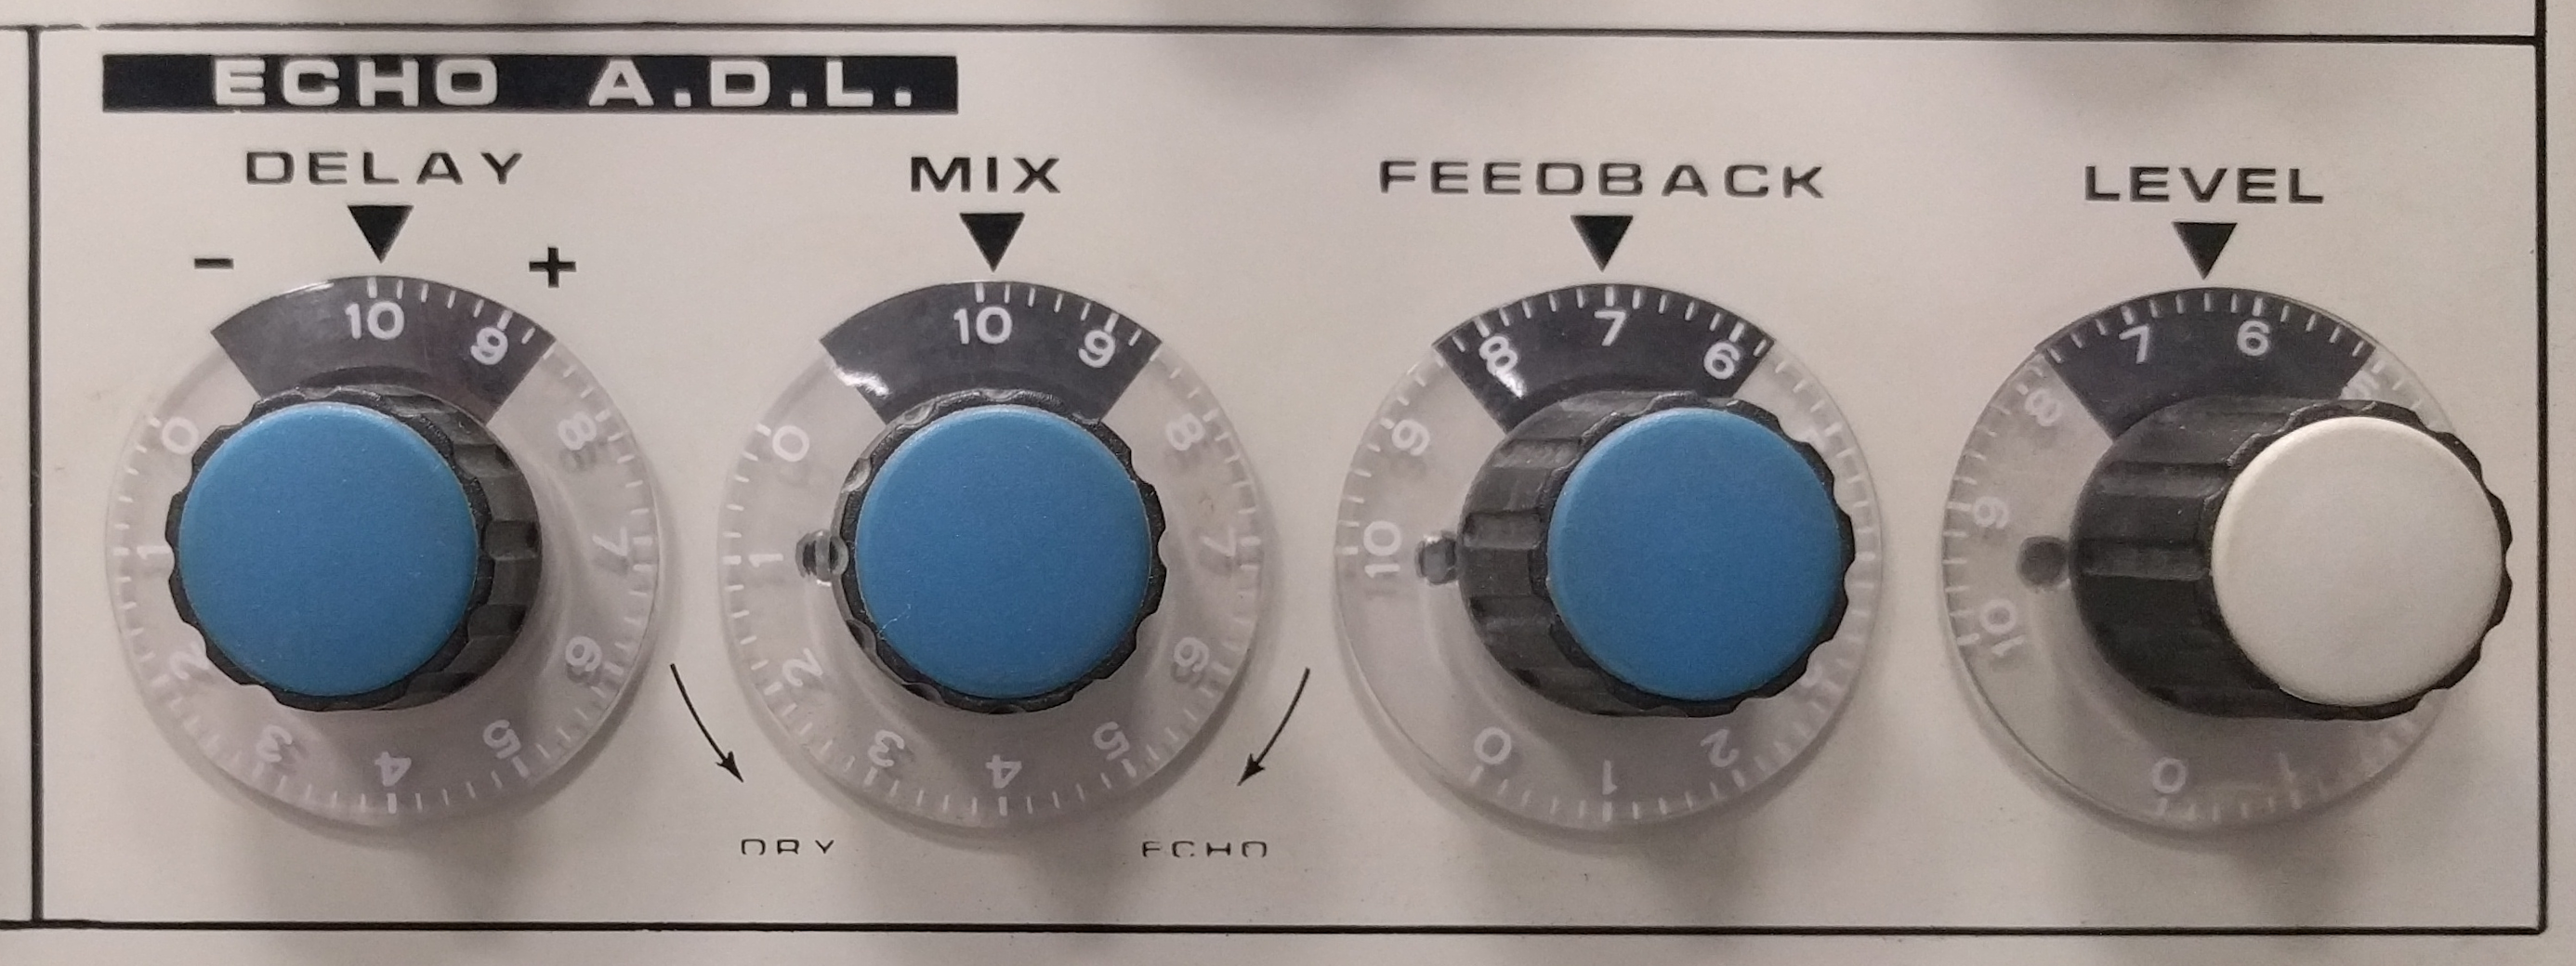
\includegraphics[width=0.7\textwidth]{images/echo}
	\caption[\textit{Echo \textsc{a. d. l.}}]{Vista del módulo \textit{Echo \textsc{a. d. l.}}.}
	\label{fig:echo}
\end{figure}

\subsection{Implementación en \appName}

Existe un \textit{UGen} en SuperCollider que emula precisamente un módulo de características similares, \texttt{SwitchDelay}. Para producir el retardo de la señal, este \textit{Ugen} posee un \textit{buffer} donde esta se almacena para ser leída en un punto variable dependiendo del tiempo de \textit{delay}. Una limitación de este sistema es, precisamente, que la variación de la cantidad de \textit{delay} en tiempo de ejecución produce artefactos debidos a los saltos abruptos del puntero de lectura. La forma encontrada de minimizar estos sonidos residuales ha consistido en hacer variar la variable de control \textit{delay} suavemente de un valor a otro con la frecuencia de muestreo. Esto suaviza notablemente los cambios de posición del puntero de lectura del \textit{buffer}, traduciéndose en una notable disminución de los ruidos, aunque no ha sido posible una eliminación absoluta de este. Es interesante seguir trabajando en la resolución de este problema ya que el delay es uno de los parámetros controlables por voltaje dentro del sintetizador.

